\documentclass{article}
\usepackage{amsmath, amssymb, amsthm}
\usepackage{enumitem}
\usepackage[margin=1in]{geometry}
\usepackage{tikz}

\title{Abstract Algebra: Homework 4}
\author{Huize Shi - A92122910}
\date {February 8, 2018}

\begin{document}
\maketitle

\section*{Section 6}

\subsection*{22. }
	Subgroup diagram of $\mathbb{Z}_{12}$\\
	\begin{tikzpicture}[node distance=2cm]
	\node(Z12) {$\mathbb{Z}_{12}$};
	\node(S2) [below left of=Z12] {$\langle 2 \rangle$};
	\node(S3) [below right of=Z12] {$\langle 3 \rangle$};
	\node(S4) [below left of=S2] {$\langle 4 \rangle$};
	\node(S6) [below right of=S2] {$\langle 6 \rangle$};
	\node(0) [below right of=S4] {$\{0\}$};

	\draw(Z12) -- (S2);
	\draw(Z12) -- (S3);
	\draw(S2) -- (S4);
	\draw(S2) -- (S6);
	\draw(S3) -- (S6);
	\draw(S4) -- (0);
	\draw(S6) -- (0);

	\end{tikzpicture}
		
\subsection*{23. }
	Subgroup diagram of $\mathbb{Z}_{36}$\\
	\begin{tikzpicture}[node distance=2cm]
	\node(Z36) {$\mathbb{Z}_{36}$};
	\node(S2) [below left of=Z36] {$\langle 2 \rangle$};
	\node(S4) [below left of=S2] {$\langle 4 \rangle$};
	\node(S6) [below right of=S2] {$\langle 6 \rangle$};
	\node(S9) [below right of=Z36] {$\langle 9 \rangle$};
	\node(S12) [below right of=S4] {$\langle 12 \rangle$};
	\node(S18) [below right of=S9] {$\langle 18 \rangle$};
	\node(0) [below right of=S12] {$\{0\}$};

	\draw(Z36) -- (S2);
	\draw(Z36) -- (S9);
	\draw(S2) -- (S4);
	\draw(S2) -- (S6);
	\draw(S4) -- (S12);
	\draw(S6) -- (S12);
	\draw(S9) -- (S18);
	\draw(S6) -- (S18);
	\draw(S12) -- (0);
	\draw(S18) -- (0);

	\end{tikzpicture}

\subsection*{24. }
	Subgroup diagram of $\mathbb{Z}_{8}$\\
	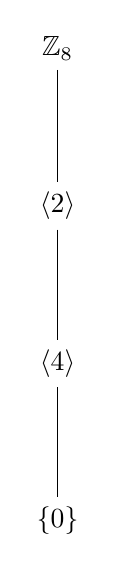
\begin{tikzpicture}[node distance=2cm]
	\node(Z8) {$\mathbb{Z}_{8}$};
	\node(S2) [below of=Z8] {$\langle 2 \rangle$};
	\node(S4) [below of=S2] {$\langle 4 \rangle$};
	\node(0) [below of=S4] {$\{0\}$};

	\draw(Z8) -- (S2);
	\draw(S2) -- (S4);
	\draw(S4) -- (0);

	\end{tikzpicture}

\subsection*{26. }
	$$<0>:\ \frac{8}{gcd(0, 8)} = 1$$
	$$<1>:\ \frac{8}{gcd(1, 8)} = 8$$
	$$<2>:\ \frac{8}{gcd(2, 8)} = 4$$
	$$<3>=<1>:\ \frac{8}{gcd(3, 8)} = 8$$
	$$<4>:\ \frac{8}{gcd(4, 8)} = 2$$
	$$<5>=<1>:\ \frac{8}{gcd(5, 8)} = 8$$
	$$<6>=<2>:\ \frac{8}{gcd(6, 8)} = 4$$
	$$<7>=<1>:\ \frac{8}{gcd(7, 8)} = 8$$
	All subgroups of $\mathbb{Z}_8$: $<0>$, $<1>$, $<2>$, $<4>$
	
\subsection*{29. }
All subgroups of $\mathbb{Z}_{17}$: $<0>$, $<1>$. 17 is prime therefore all
number from 1 to 16 are prime to 17. This means the only subgroups are $<0>$ and
$<1>$

\subsection*{45. }
\begin{proof}
Let r and s be positive integers. Show that $\{nr + ms \mid n, m \in
	\mathbb{Z}\}$ is a subgroup of $\mathbb{Z}$
	\paragraph{Closure: } 
		\begin{align*}
			&(n_1r+m_1s) + (n_2r+m_2s)\\
			=& n_1r+ n_2r + m_1s + m_2s\\
			=& (n_1+ n_2)r + (m_1 + m_2)s\\
		\end{align*}
		Hence show the set is closed under addition.

	\paragraph{Identity: }
		$$(0r+0s) = 0$$
		Hence shown 0 is in the set.

	\paragraph{Inverse: }$\forall \{nr + ms \mid n, m \in \mathbb{Z}\}$, let the
	inverse be defined as $\{(-n)r + (-m)s \mid n, m \in \mathbb{Z}\}$.
		\begin{align*}
			&(nr + ms) + ((-n)r + (-m)s)\\
			=& nr - nr + ms - ms\\
			=& 0
		\end{align*}
	Hence shown that $\{nr + ms \mid n, m \in \mathbb{Z}\}$ is a subgroup of
	$\mathbb{Z}$.
\end{proof}

\subsection*{50. }
\begin{proof} Since a is of order 2, $a^2 = a*a = e$. Consider the following: 
\begin{align*}
	&(xax^{-1})^2\\
	=& (xax^{-1})(xax^{-1})\\
	=& xa(x^{-1}x)ax^{-1}\\
	=& x((ae)a)x^{-1}\\
	=& xx^{-1}\\
	=& e
\end{align*}
It is evident that $xax^{-1} \neq e$ because it would imply that $a=e$ which is
of order 1. Since a is the unique element that has order 2, and
$(xax^{-1})^2=e$, this imply that $xax^{-1}=a$, because no other element when
raised to the second power would evaluates to e. Therefore the following holds:
\begin{align*}
	xax^{-1}&=a\\
	xa(x^{-1}x)&=ax\\
	xae&=ax\\
	xa&=ax\\
\end{align*}
\end{proof} 

\subsection*{51. }
Generators of $\mathbb{Z}_{pq}$ are defined as integers that are less than pq
and are relatively prime to pq. Since there are $(p-1)$ number of multiples of
q, and $(q-1)$ number of multiples of p, there are $(pq-1) - (p-1) - (q-1)$
number of integers that are less than pq and relatively prime to pq.
	\begin{align*}
		&(pq-1) - (p-1) - (q-1)\\
		=& pq-1 - p+1 - q+1\\
		=& pq - p - q+1 \\
		=& (p-1)(q-1)
	\end{align*}
	There are $(p-1)(q-1)$ number of positive integers that generates
	$\mathbb{Z}_{pq}$.

\subsection*{52. }
Let p be a prime number and r an integer $\ge 1$. There are $p^{r-1}-1$ factors
of $p^r$. There are $p^r - 1$ number s less than $p^r$. The number of coprime
integers less than $p^r$ is as follows: 
	\begin{align*}
		&(p^r-1) - (p^{r-1} - 1)\\
		=& p^r-1 - p^{r-1} + 1\\
		=& p^r - p^{r-1}\\
		=& p^{r-1}(p-1)
	\end{align*}
	There are $p^{r-1}(p-1)$ number of generators of the cyclic group
	$\mathbb{Z}_{p^r}$ where p is a prime number and r is an integer $\ge 1$.

\subsection*{55. }
\begin{proof}
	Cyclic group $C \le G$ is the smallest possible subgroups. This means that if
	there exist a nontrivial proper subgroup, it must be a cyclic group of G. Given
	$\mathbb{Z}_p$ where p is a prime number. All $p-1$ numbers less than p are
	coprime to p. this means that all $p-1$ generators generates G which means that
	there are no proper nontrivial subgroup of $\mathbb{Z}_p$ if p is a prime
	number.
\end{proof}

\subsection*{56. }
\paragraph{a. } Let $H=<a>$ and $K=<b>$. Since $|H|=r$ and $|k|=s$, we know that
because G is abelian $(ab)^{rs}=(a^r)^s(b^s)^r=e$. Guessing that $<ab>$
generates the cyclic subgroup of order rs.
\subparagraph{Identity: } 
\begin{align*}
	(ab)^n &= e\\
	a^nb^n &= e\\
	a^n &= b^{-n} = c
\end{align*}
Since c is in H and K, it generates subgroup of H with some order that divides
r, and also generates subgroup of K with some order that divides s. However,
since r and s are coprimes, the following is implied: 
	$$(|<c>| = 1) \Rightarrow (<c>={e}) \Rightarrow (c=e)$$
Hence we know $a^n = b^{-n} = e$, this means that since $a^n \in H$ and $b^n \in
K$, this means n must be divisible by both r and s. Hence we know $n = rs$. This
means that $<ab>$ is the subgroup of order rs.

\paragraph{b. } Let $m=gcd(r, s)$, $n = mp$ and p is prime to r and that $rp =
rs/m$ is the LCM(r, s). This means that $|<a>|=r \wedge |<b^m>|=p$. Since r and
q are coprimes, by part a, we know that $ab^d$ generates the cyclic subgroup of
order the LCM of r and s.

\end{document}

